%! Author = Jan
%! Date = 13.05.2022

\section*{Defusing Bombs}
\rhead{Defusing Bombs}
A bomb will explode when its countdown timer reaches 0:00 or when too
many strikes have been recorded. The only way to defuse a bomb is to disarm
all of its modules before its countdown timer expires.

\begin{figure}[h]
  \centering
  \caption*{Example Bomb}
  \begin{minipage}{.4\textwidth}
    \centering
    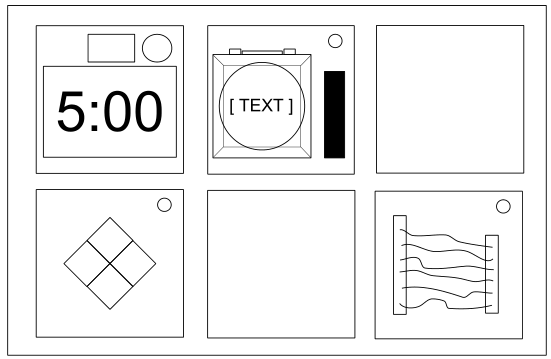
\includegraphics[height=4.5cm]{modules/0_explanation/bomb_front}
    \caption*{Front}
    \label{fig:sub1}
  \end{minipage}%
  \begin{minipage}{.3\textwidth}
    \centering
    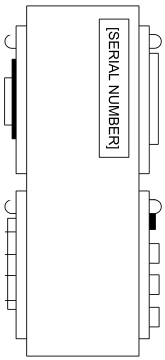
\includegraphics[height=4.5cm]{modules/0_explanation/bomb_side}
    \caption*{Side}
    \label{fig:sub2}
  \end{minipage}
  \label{fig:example_bomb}
\end{figure}

\subsection*{Modules}
Each bomb will include one or several modules that must be disarmed. Each
module is discrete, but some modules require to be solved before others.


Instructions for disarming modules can be found in Section 1.
"Needy" modules present a special case and are described in Section 2.

\subsection*{Strikes}
\begin{wrapfigure}[7]{r}{0.2\textwidth} %this figure will be at the right
  \vspace{-2\baselineskip}
  Strike Indicator
  \centering
  
\includegraphics[height=3.5cm]{modules/0_explanation/strike}
  \label{fig:Strikes}
\end{wrapfigure}
When the Defuser makes a mistake the bomb will record a strike
which will be displayed on the indicator above the countdown
timer. Bombs with a strike indicator will explode upon the
third strike. The timer will begin to count down faster after
a strike has been recorded.

If no strike indicator is present above the countdown timer,
the bomb will explode upon the first strike, leaving no room
for error.

\subsection*{Gathering Information}
Some disarming instructions will require specific information about the
bomb, such as the serial number. For detailed descriptions see the next
page "On the Subject of Edgework".

\clearpage
